\documentclass{wit-slides-2020}

\usepackage{relsize}

\begin{document}

\maketitle

\section{Module Introduction}

%% ======================
\begin{frame}[label=todo]{Aim of Module}

\begin{enumerate}
	\item
	Develop a working knowledge of:
	\begin{itemize}
	\item networks and data communications.
	\item operating systems and virtualisation solutions.
	\item Linux terminal interface, such as for data retrieval, text file manipulation, and scripting.
	\item modern programming languages (such as Python) in the retrieval and analysis of scientific data.
	\end{itemize}
	\item
	Build, configure and manage essential network infrastructure and application services. 	
	\item
	Construct a pipeline of different programs that automates collation, analysis, and reporting of data.
\end{enumerate}

\vspace{-6pt}

\begin{center}
\tikz\node[law,align=left, text width=11cm] {\centerline{\textcolor{structure}{Informal Aim}}\\[-6pt]Given a task:\\1) determine required software to address problem,\\ 2) {\bf independently} investigate, build, configure and use selected software to solve problem, and\\ 3) generate suitable reports};
\end{center}
\end{frame}

\begin{frame}{What? (and Who?)}
\vspace*{-2em}\begin{center}
\hspace*{-1.25em}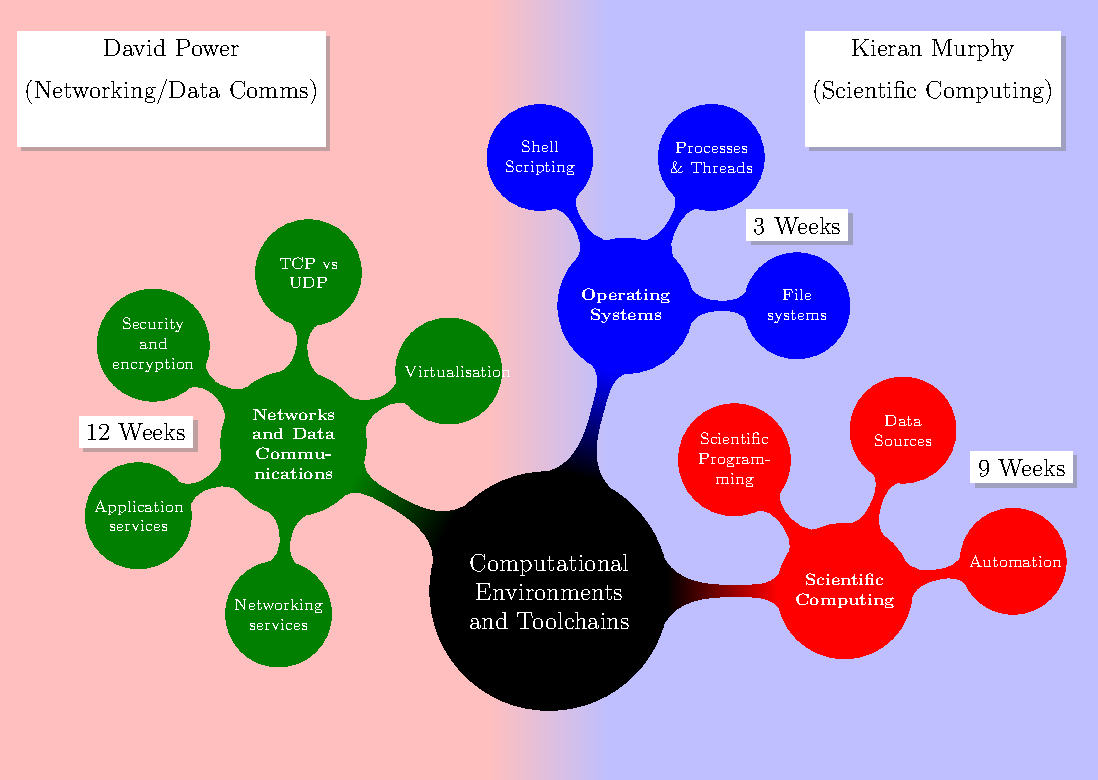
\includegraphics[page=1,height=.9\paperheight, width=12.8cm]{../../../shared/mindmap/mindmaps}
\end{center}
\end{frame}
%% ======================

%% ======================
\begin{frame}[label=todo]{Why?}

This is a relatively new module\footnote{adopted from the existing Data Communications module shared with the BSc in Applied Computing students.} to address particular needs of Physics students in light of recent trends in the scientific computing world.
\begin{itemize}
\item
Increasing use of virtualisation (and containerisation) to address networking, instantiation of compute nodes and services, and avoiding cross-platform porting of software.
\item
Industry, following the academic community, is moving from propriatorey to open source software for computational needs \ldots
\begin{itemize}
\item 
Computational Languages: \\
MATLAB, Mathematica, Maple\hfill $\to$\hfill Octave, {\bf Python}, SCILAB
\item
Statistics, Data analytics:\\
SPSS, SAS \hfill$\to$\hfill {\bf Python}, R
\item
Documentation generation, version control, etc
\end{itemize}
\item
Scientific community is moving towards reproducible research\footnote{\scriptsize 10 Simple Rules for the Care and Feeding of Scientific Data (\url{arxiv.org/abs/1401.2134})}
 --- where both data and the code used in the analysis is also published.

\end{itemize}

\end{frame}
%% ======================



%======================================
%@FRAME ---
%======================================
\begin{frame}{A Computational Physicist needs to Know Everything \ldots}

\vspace{-10pt}\hspace*{-.4cm}
\centerline{\includegraphics[page=2,width=.96\textwidth,clip,trim=0 0 0 0]{/wit/modules/Computational_Physics/shared/map/map.pdf}}
\end{frame}
%======================================
%\note{}

%% ======================
\begin{frame}[label=todo]{How?}

\minisec{Contact hours}\vspace{6pt}

Two 2-hour lecture/practical sessions per week \dotfill (KM / DP)

\vspace{6pt}
\centerline{\tikz\node[law,scale=1]{%
\smaller David will talk to you about his approach for his lecture/practical sessions.
};}

\vspace{6pt}
In terms of my sessions (Tue 9:15--11:15):
\begin{itemize}
%\item Initially we will keep to same time slots, but I'm happy to move them around to suit the class as long as it does not clash with other commitments 

\item Aim to structure lecture/practical sessions as:
\begin{itemize}
	\item 
	Emphasis on practical work ({\bf read theory in own time}).
	\item
	Single/double practical for individual technology/topic/case study.
\end{itemize}
\end{itemize}


\end{frame}
%% ======================

%% ======================
\begin{frame}[label=todo]{Learning Technologies}

\minisec{Moodle: \href{https://moodle.wit.ie/course/view.php?id=209166&section=1}{moodle.wit.ie}}
\hfill \raisebox{6pt}[0pt][0pt]{
\includegraphics[trim=0 0 0 0,scale=.3]{pic/Moodle}}

\vspace{-9pt}
\begin{itemize}
\item
Launch point for module material. 
\item 
All assignments and module deliverables.
\item
Will copy-post from slack important message here.
\end{itemize}

\vspace{6pt}
\minisec{Website: \href
{https://setu-ceandt.github.io/live}
{setu-ceandt.github.io/live}
}
\hfill \raisebox{9pt}[0pt][0pt]{
\includegraphics[trim=0 0 0 0,width=1.5cm]{pic/Github}}

\vspace{-9pt}
\begin{itemize}
\item
Location of module content.
\item
Links to deliverables.
\end{itemize}

\vspace{6pt}
\minisec{Google's Colab: 
\href{https://colab.research.google.com/notebooks/intro.ipynb}{colab.research.google.com}
}
\hfill \raisebox{6pt}[0pt][0pt]{
\includegraphics[trim=0 0 0 0,scale=.06]{pic/colab}}

\vspace{-9pt}
\begin{itemize}
\item
You can use your own  instance of python (I prefer anaconda) and the Jupyter interface. However, to simplify things this semester I'm going to use Google's colab interface when working with python notebooks.
\end{itemize}

\vspace{6pt}
\minisec{Slack: 
\href{https://ceandt202425.slack.com}{ceandt202425.slack.com}
}
\hfill \raisebox{9pt}[0pt][0pt]{
\includegraphics[scale=.02]{pic/slack}}

\vspace{-12pt}
\begin{itemize}
\item
Used for instant messaging, one-on-one sessions, etc.
\end{itemize}
\end{frame}
%% ======================

%% ======================
\begin{frame}[label=todo]{Assessment Structure}

Module is 100\% CA with 50\% for Networking (DP) and 50\% for Scientific Computing (KM).

\vspace{6pt}
\centerline{\tikz\node[law,scale=1]{%
\smaller David will talk to you about his approach for 50\% for Networking.
};}

In terms of my 50\%:

\minisec{Participation during in-class practicals, 20\%}
\vspace{3pt}

%{\smaller[2]\it Taking online course requires more effort to actively manage one's participation and avoiding falling behind in the course work.  
%In recognition of this I'm willing to allocate 20\% of the module grade to deliverables that are intended to encourage participation rather than focusing on testing competency.
%
%}

\begin{itemize}
\item Student notebooks based on practical sessions.
\end{itemize}

\minisec{Computational Tasks, 80\%}

\vspace{6pt}
Weekly assignment activity (default due on Saturday @ 23:00):

\begin{enumerate}
\item Moodle quizzes (Computational)
\item 4--5 Computational tasks (current plan)
\item Grade based on:
\begin{itemize}
\item Level of specification that was satisfied
\item Analysis/programming quality
\end{itemize}
\end{enumerate}

\end{frame}
%% ======================


%%% ======================
%\begin{frame}[label=todo]{Academic Integrity}
%
%\minisec{Official statement}\vspace{6pt}{\smaller
%The School of Science \& Computing at Waterford Institute of Technology is committed to maintaining the highest standards of academic integrity. Academic misconduct, including but not limited to cheating may result in a mark of zero for the assignment as well as disciplinary action. Plagiarism or cheating may impact your grant if you receive one. Additional sanctions may by imposed depending on the case. You are responsible for adhering to all regulations regarding academic integrity. When in doubt about whether something is plagiarism, please see the guidelines published on the \href{https://www.wit.ie/current_students/student_affairs/Exam_Procedures_Regulations}{WIT website}. ''
%
%}
%
%\vfill
%\minisec{My comments or `lessons learnt from going online in Spring 2020'}
%\vspace{6pt}\smaller
%\begin{itemize}
%\item
%I have been involved in two cases of plagiarism in the summer exam sessions and it is not pleasant. 
%\item
%Crossing the line from giving/receiving help to plagiarism is easy.  So follow the rule of `writing every line of code yourself' (even if you are getting significant guidance from other sources) and make sure you can explain every line.  
%\item
%Most lectures will probably have an interview component to grading near end of semester.  
%\end{itemize}
%
%\end{frame}
%%% ======================
%


%%% ======================
%\begin{frame}[label=todo]{Netiquette}
%
%{\small\it
%Remote learning can be taxing on the Student as well as the Lecturer. To assist with this, certain behaviours and standards are expected for online sessions with this module. When engaging with synchronous (e.g. live, real-time) remote classes
%
%}
%
%\begin{itemize}
%\item Find quiet place free from distractions (siblings, pets, parents, television, etc).
%\item You will need writing materials for taking notes --- you will not be able to record notes on a computer in real-time.
%\item Use headphones, mute your microphone and turn your camera on:
%\begin{itemize}
%\item Video on encourages more active participation and promotes focus.  
%\item Zoom has a walkie-talkie feature --- press and hold space bar while talking to be heard.
%\end{itemize}
%\item Be respectful to your classmates and lecturers when speaking/writing.
%\item Attendance will be taken in every class.
%\end{itemize}
%\end{frame}
%%% ======================



%% ======================
\begin{frame}[label=todo]{Background Reading (OS \& Scientific Computing)}

We will put up more texts later in the module, but just in case you are looking for some light reading to get you started have a look at these \ldots

\vspace{6pt}
\footnotesize
\begin{minipage}{.15\textwidth}

\includegraphics[width=\textwidth]{Effective_Computation_in_Physics}
\end{minipage}
\hfill
\begin{minipage}{.8\textwidth}
{\bf Effective Computation in Physics}\\
by Anthony Scopatz \& Kathryn Huff\\
Touches on nearly all of the topics that we hope to cover in the Scientific Computing part of the course.  Well worth buying.
\end{minipage}

\vspace{-12pt}
\begin{minipage}{.8\textwidth}
{\bf Python Scripting for Computational Science}\\
by Hans Petter Langtangen\\
Chapters 1 to 4 give a good coverage of the Python language, later chapters cover interfacing python with C/C++ (not needed). 
\end{minipage}
\begin{minipage}{.15\textwidth}

\includegraphics[width=\textwidth]{Python_Scripting_for_Computational_Science}
\end{minipage}

\vspace{-12pt}
\begin{minipage}{.15\textwidth}
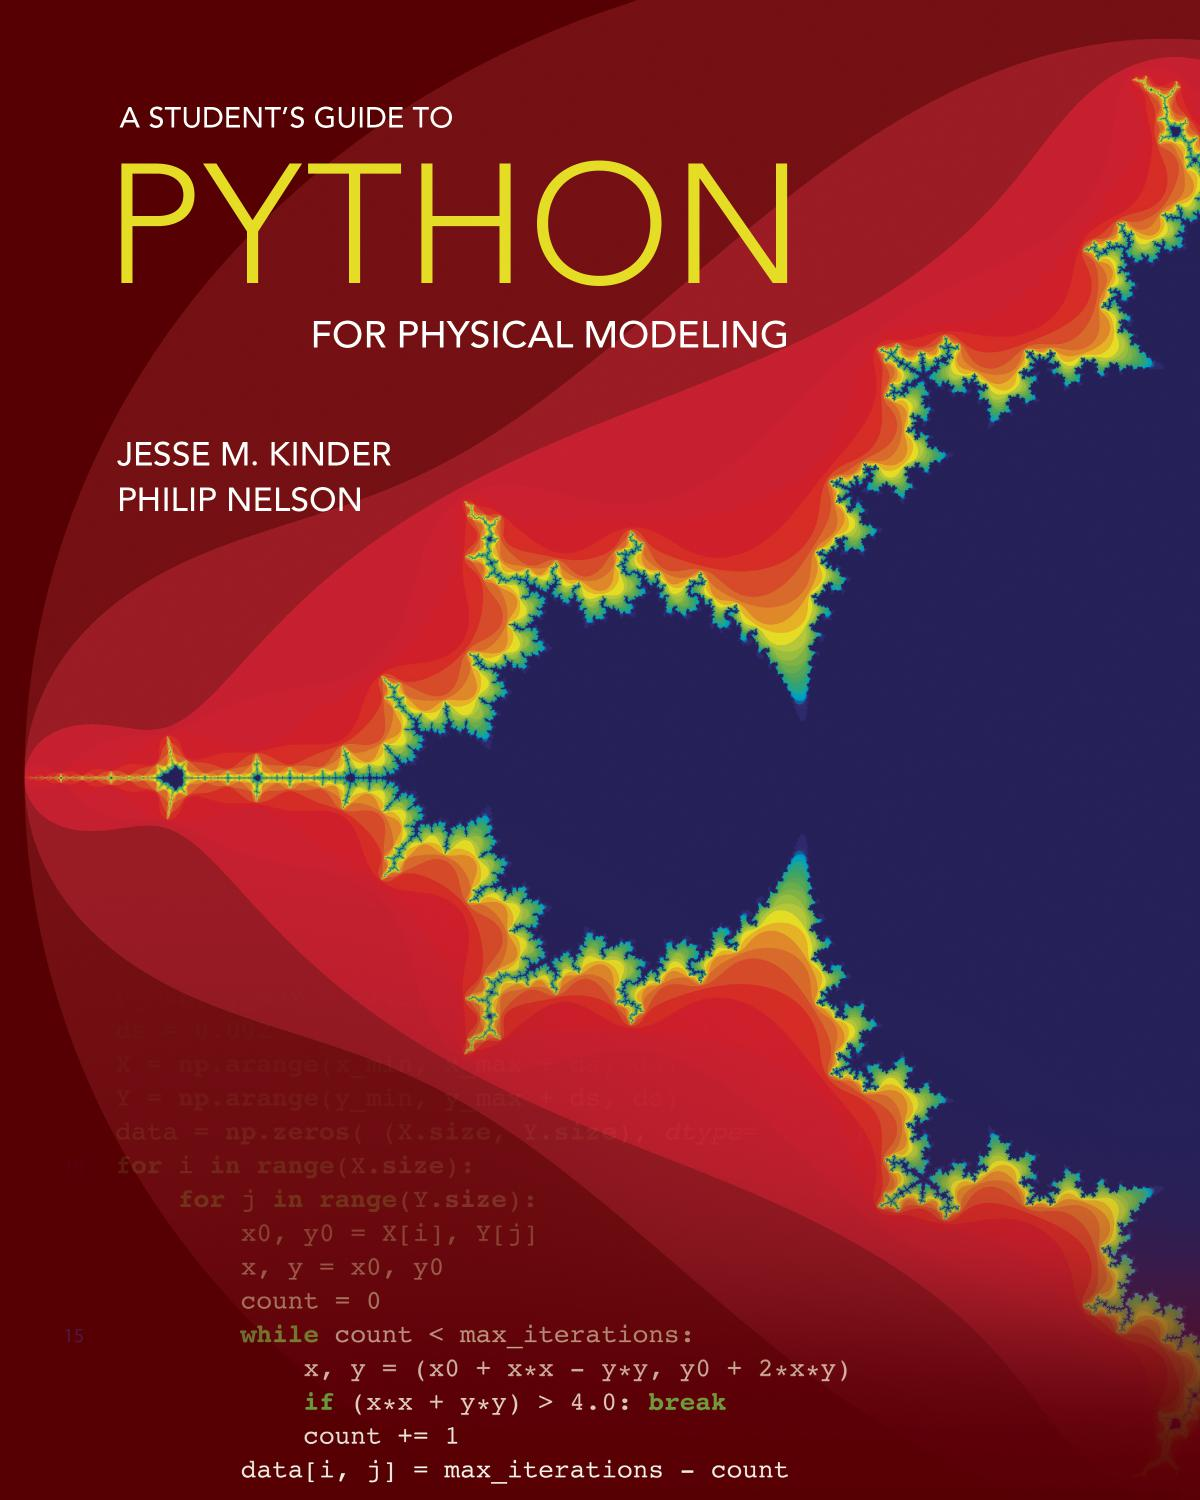
\includegraphics[width=\textwidth]{Students_Python_Guide}
\end{minipage}
\hfill
\begin{minipage}{.8\textwidth}
{\bf Student's Python Guide}\\
by Jesse M. Kinder \& Philip Nelson\\
Good overview of python and we will probably base some of our practicals on those covered in this book.
\end{minipage}

\end{frame}
%% ======================

%% ======================
\begin{frame}[label=todo]{Today's (W01) task --- getting used to python/colab \ldots}

\begin{center}
\begin{tikzpicture}
\node[draw, fill=white, rounded corners=12pt, drop shadow]
{\href{https://colab.research.google.com/github/kmurphy/kmurphy.github.io/blob/master/notebooks/CEandT_Blank.ipynb}{
\includegraphics[width=5cm]{colab}}};
\end{tikzpicture}
\end{center}
\end{frame}
%% ======================

%% ======================
\begin{frame}[label=todo]{Today's (W01) assignment --- python hour of code activity}

\begin{center}
\begin{tikzpicture}
\node[draw, fill=white, rounded corners=12pt, drop shadow]
{\href{https://hourofcode.com/toxicodecompute2}{
\includegraphics[width=5cm]{toxicode_compute2.jpg}}};
\end{tikzpicture}

\vspace{12pt}

\ldots\ and Moodle assignment link to upload progress \ldots

\vspace{15pt}
\begin{tikzpicture}
\node[draw, fill=white, rounded corners=12pt, drop shadow]
{\href{https://moodle.wit.ie/mod/assign/view.php?id=4341236}{
\includegraphics[width=3cm]{Moodle.png}}};
\end{tikzpicture}
\end{center}

\end{frame}
%% ======================

\end{document}